\documentclass[12pt]{article}
\usepackage{amsmath}
\usepackage{amsfonts}
\usepackage{parskip}
\usepackage{amsthm}
\usepackage{thmtools}
\usepackage[headheight=15pt]{geometry}
\geometry{a4paper, left=20mm, right=20mm, top=30mm, bottom=30mm}
\usepackage{graphicx}
\usepackage{bm} % for bold font in math mode - command is \bm{text}
\usepackage{enumitem}
\usepackage{fancyhdr}
\usepackage{amssymb} % for stacked arrows and other shit
\pagestyle{fancy}
\usepackage{changepage}
\usepackage{mathcomp}
\usepackage{tcolorbox}

\declaretheoremstyle[headfont=\normalfont]{normal}
\declaretheorem[style=normal]{Theorem}
\declaretheorem[style=normal]{Proposition}
\declaretheorem[style=normal]{Lemma}
\newcounter{ProofCounter}
\newcounter{ClaimCounter}[ProofCounter]
\newcounter{SubClaimCounter}[ClaimCounter]
\newenvironment{Proof}{\stepcounter{ProofCounter}\textsc{Proof.}}{\hfill$\square$}
\newenvironment{Solution}{\stepcounter{ProofCounter}\textbf{Solution:}}{\hfill$\square$}
\newenvironment{claim}[1]{\vspace{1mm}\stepcounter{ClaimCounter}\par\noindent\underline{\bf Claim \theClaimCounter:}\space#1}{}
\newenvironment{claimproof}[1]{\par\noindent\underline{Proof of claim \theClaimCounter:}\space#1}{\hfill $\blacksquare$ Claim \theClaimCounter}
\newenvironment{subclaim}[1]{\stepcounter{SubClaimCounter}\par\noindent\emph{Subclaim \theClaimCounter.\theSubClaimCounter:}\space#1}{}
% \newenvironment{subclaimproof}[1]{\begin{adjustwidth}{2em}{0pt}\par\noindent\emph{Proof of subclaim \theClaimCounter.\theSubClaimCounter:}\space#1}{\hfill
% $\blacksquare$ \emph{Subclaim \theClaimCounter.\theSubClaimCounter}\vspace{5mm}\end{adjustwidth}}
\newenvironment{subclaimproof}[1]{\par\noindent\emph{Proof of subclaim \theClaimCounter.\theSubClaimCounter:}\space#1}{\hfill
$\Diamond$ \emph{Subclaim \theClaimCounter.\theSubClaimCounter}}

\allowdisplaybreaks{}

% chktex-file 3

\title{STAT 643: HW 4}
\author{Evan P. Walsh}
\makeatletter
\makeatother
\lhead{Evan P. Walsh}
\chead{STAT 643: HW 4}
\rhead{\thepage}
\cfoot{}

\begin{document}
\maketitle


\newcommand{\E}{\mathrm{E}}
\renewcommand{\baselinestretch}{1}

\subsection*{1}
\begin{tcolorbox}
  Consider the two-state decision problem with $\Theta=\{1,2\}$ and $P_1$ as the Bernoulli$(1/4)$ distribution and
  $P_2$ as the Bernoulli$(1/2)$ distribution. Let $\mathcal{A}=\Theta$ and $L(\theta,a)=I(\theta \neq a)$.
  \begin{enumerate}
    \item[(a)] Find $\mathcal{S}^0$, the set of risk vectors (risk points in $\mathbb{R}^2$) for the four possible non-randomized decision rules here.  Plot these risk points in the plane and then sketch $\mathcal{S}$, the set of all randomized risk vectors.
    \item[(b)] Identify $A(\mathcal{S})$, the set of all admissible risk vectors.  Is there a minimal complete class for this decision problem? If there is one, what is it?  (Note: It can be shown through direct, but tedious, calculation that any element of $\mathcal{D}^*$ has a corresponding element of $\mathcal{D}_*$ with the same risk vector, and vice versa.  You may use this fact without proof. In the finite geometry decision framework, we used randomized rules $\mathcal{D}_*$ and, in discussing complete classes, we used behavioral rules $\mathcal{D}^*$; but this difference generally doesn't matter, in this problem in particular.)
  \end{enumerate}
\end{tcolorbox}
\begin{Solution}
  \begin{figure}[h!]
    \centering
    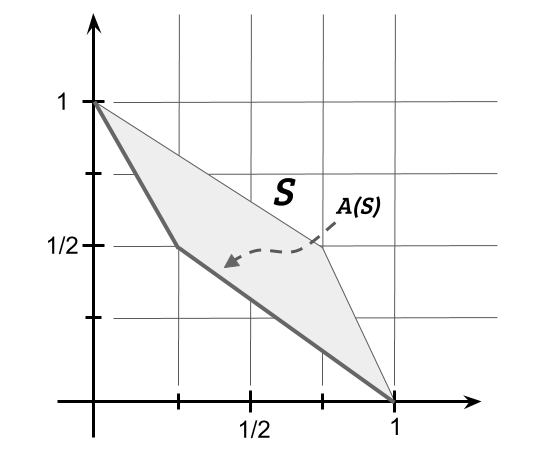
\includegraphics[width=0.5\textwidth]{./figures/hw04.png}
    \caption{Risk vectors. The bottom boundary of the polygon given by the thicker line representst the set of admissible rick vectors.}
    \label{fig:1}
  \end{figure}


  (a) The four possible non-randomized decision rules are given by 
  \[ 
    \delta_1(x) := \left\{ \begin{array}{cl} 1 & \text{ if } x = 0 \\ 1 & \text{ if } x = 1 \end{array} \right. \qquad 
    \delta_2(x) := \left\{ \begin{array}{cl} 1 & \text{ if } x = 0 \\ 2 & \text{ if } x = 1 \end{array} \right. 
  \]
  \[ 
    \delta_3(x) := \left\{ \begin{array}{cl} 2 & \text{ if } x = 0 \\ 1 & \text{ if } x = 1 \end{array} \right. \qquad 
    \delta_4(x) := \left\{ \begin{array}{cl} 2 & \text{ if } x = 0 \\ 2 & \text{ if } x = 1 \end{array} \right. 
  \]

  We can then calculate the risk associated with each one as 
  \begin{align*}
    R(1, \delta_1) & = E_{1}I(1 \neq \delta_1) = P_{1}(1 \neq \delta_1) = 0 \\
    R(2, \delta_1) & = P_{2}(2 \neq \delta_1) = 1 \\
    R(1, \delta_2) & = P_{1}(1 \neq \delta_2) = 1/4 \\
    R(2, \delta_2) & = P_{2}(1 \neq \delta_2) = 1/2 \\
    R(1, \delta_3) & = P_{1}(1 \neq \delta_3) = 3/4 \\
    R(2, \delta_3) & = P_{2}(1 \neq \delta_3) = 1/2 \\
    R(1, \delta_4) & = P_{1}(1 \neq \delta_4) = 1 \\
    R(2, \delta_4) & = P_{2}(1 \neq \delta_4) = 0 \\
  \end{align*}

  Thus, the corresponding points in $\mathbb{R}^2$ of the risk vectors associated with each rule are 
  \[
    (0,1) \text{ for } \delta_1, \qquad (1/4, 1/2) \text{ for } \delta_2, \qquad (3/4, 1/2) \text{ for } \delta_3, \qquad \text{ and } (1, 0) \text{
    for } \delta_4.
  \]
  These are the corners of the polygon in Figure \ref{fig:1}. The polygon itself makes up $S$, the set of risk vectors for all randomized decision
  rules, since $S$ is the convex hull of the non-randomized risk vectors. \\

  (b) The set of all admissible rick vectors, $A(\mathcal{S})$, is given by the thick lower sides of the polygon in Figure \ref{fig:1}. We also claim that
  $A(\mathcal{S})$ is a minimal complete class. Well, clearly $A(\mathcal{S})$ is a complete class. Thus, by Theorem 64, $A(\mathcal{D}^{*})$ is
  minimal complete. But $A(\mathcal{D}^*) = A(\mathcal{S})$.

\end{Solution}

\subsection*{2}
\begin{tcolorbox}
Consider the two-state decision problem with $\Theta=\{1,2\}$, where the observable $X=(X_1,X_2)$ has iid Bernoulli$(1/4)$
  components when $\theta=1$ and  has iid Bernoulli$(1/2)$
  components when $\theta=2$. Let $\mathcal{A}=\Theta$ and $L(\theta,a)=I(\theta \neq a)$.  Consider the behavioral decision rule $\phi$, with $\phi_x\equiv \phi_{(x_1,x_2)}$, defined as
  \begin{eqnarray*}
    \phi_x(\{1\})=1 &\mbox{if $x_1=0$}\\
    \phi_x(\{1\})=1/2 &\mbox{if $x_1=1$}
  \end{eqnarray*}

  \begin{enumerate}
    \item Show that $\phi$ is inadmissible by finding a decision rule with a better risk function.

    \item Find a behavioral decision rule that is a function of the sufficient statistic $T(X)=X_1+X_2$ and is risk equivalent to $\phi$.

  \end{enumerate}
\end{tcolorbox}

\begin{Solution}
  Let $x = (x_1, x_2)$.  \\
  
  (a) For $\theta = 1$, the risk of $\phi$ is given by 
  \begin{align*}
    R(1, \phi) = \int_{\mathcal{X}}\int_{\mathcal{A}} L(1, a)d\phi_{x}(a)dP_1(x) & = \sum_{x \in \{0,1\}^2} \phi_x(\{a \neq 1\}) P_1(X_1=x_1)P_1(X_2 =
    x_2) \\
    & = (1/2)(1/4)(3/4) + (1/2)(3/4)(3/4) = 3/8,
  \end{align*}
  and similarly for $\theta = 2$,
  \begin{align*}
    R(2,\phi) = \int_{\mathcal{X}}\int_{\mathcal{A}} L(2, a)d\phi_{x}(a)dP_2(x) & = \sum_{x \in \{0,1\}^2} \phi_x(\{a \neq 2\}) P_2(X_1=x_1)P_2(X_2 =
    x_2) \\
    & = (1/2)^2 + (1/2)^2 + (1/2)^3 + (1/2)^3 = 3/4.
  \end{align*}
  Now, set 
  \[
    \phi_x'(\{1\}) := \left\{ \begin{array}{cl} 1 & \text{ if } x_1 = x_2 \\ 1/2 & \text{ if } x_1 \neq x_2. \end{array} \right. 
  \]
  Then, similar to the calculations above, we find that for $\theta = 1$, the risk of $\phi'$ is given by 
  \begin{align*}
    R(1, \phi') = \int_{\mathcal{X}}\int_{\mathcal{A}} L(1, a)d\phi_{x}'(a)dP_1(x) & = \sum_{x \in \{0,1\}^2} \phi_x'(\{a \neq 1\}) P_1(X_1=x_1)P_1(X_2 =
    x_2) \\
    & = (1/2)(3/16) + (1/2)(3/16) \\
    & = 3/16 < 3/8 = R(1,\phi)
  \end{align*}
  and for $\theta = 2$,
  \begin{align*}
    R(2,\phi') = \int_{\mathcal{X}}\int_{\mathcal{A}} L(2, a)d\phi_{x}'(a)dP_2(x) & = \sum_{x \in \{0,1\}^2} \phi_x'(\{a \neq 2\}) P_2(X_1=x_1)P_2(X_2 =
    x_2) \\
    & = (1/4) + (1/2)(1/4) + (1/2)(1/4) + (1/4) \\
    & = 3/4 = R(2, \phi).
  \end{align*}
  Hence $\phi'$ is better than $\phi$, so $\phi$ is inadmissible. \\

  (b) Take $\phi_x'(\{1\}) := 3/4$ for all $x \in \{0,1\}^2$. Then clearly $\phi_x' \equiv \phi_T'$ is a function of $T$, and 
  \begin{align*}
    R(1, \phi') = \int_{\mathcal{X}}\int_{\mathcal{A}} L(1, a)d\phi_{x}'(a)dP_1(x) & = \sum_{x \in \{0,1\}^2} \phi_x'(\{a \neq 1\}) P_1(X_1=x_1)P_1(X_2 =
    x_2) \\
    & = (1/4)(9/16) + (1/4)(3/16) + (1/4)(3/16) + (1/4)(9/16) \\
    & = 3/8 = R(1, \phi),
  \end{align*}
  and 
  \begin{align*}
    R(2,\phi') = \int_{\mathcal{X}}\int_{\mathcal{A}} L(2, a)d\phi_{x}'(a)dP_2(x) & = \sum_{x \in \{0,1\}^2} \phi_x'(\{a \neq 2\}) P_2(X_1=x_1)P_2(X_2 =
    x_2) \\
    & = (3/4)(1/4) + (3/4)(1/4) + (3/4)(1/4) + (3/4)(1/4) \\
    & = 3/4 = R(2,\phi).
  \end{align*}
  Thus $\phi'$ and $\phi$ are risk equivalent.
\end{Solution}


\subsection*{3}
\begin{tcolorbox}
  Let $X_1,\ldots,X_n$ be iid binary random variables with $P_\theta(X_1=1)=\theta=1-P_\theta(X_1=0)$ for $\theta \in(0,1)$.  Consider estimating $\theta$ based on squared error loss and $X=(X_1,\ldots,X_n)$.  Derive the risk functions of the following estimators:
  \begin{enumerate}
    \item the non-randomized rules $\bar{X}$ (sample mean of $X$) and
      \[
        T_0(X) = \left\{\begin{array}{lcl}
            0 && \mbox{if more than half of the $X_i$'s are 0}\\
            1 && \mbox{if more than half of the $X_i$'s are 1}\\
            0.5 && \mbox{if exactly half of the $X_i$'s are 0}
        \end{array}\right.
      \]
      It suffices to express risks for $T_0(X)$ in terms of probabilities involving $\bar{X}$.
    \item the decision rules (involving forms of randomization) given by
      \[
        T_1(X) = \left\{\begin{array}{lcl}
            \bar{X} && \mbox{w.p. $0.5$}\\
            T_0(X) &&  \mbox{w.p. $0.5$}
        \end{array}\right. \quad \& \quad  T_2(X) = \left\{\begin{array}{lcl}
            \bar{X} && \mbox{w.p. $\bar{X}$}\\
            0.5 &&  \mbox{w.p. $1-\bar{X}$}
        \end{array}\right.
      \]
  \end{enumerate}
\end{tcolorbox}

\begin{Solution}
  Let $Y := \sum_{i=1}^{n}X_{i}$ so that $Y$ is Binomial$(n, \theta)$. Let $\theta \in (0,1)$. Then 
  \begin{align*}
    R(\theta, \bar{X}) = E_{\theta}(\theta - \bar{X})^{2} & = Var_{\theta}\left[ \bar{X} \right] + [\text{Bias}_{\theta}(\bar{X})]^{2} =
    \frac{\theta(1-\theta)}{n}.
  \end{align*}
  Define $q_1(\theta) := P_{\theta}\left( Y < \frac{n}{2} \right)$, $q_2(\theta) := P_{\theta}\left( Y > \frac{n}{2} \right)$, and $q_3(\theta) := 1 -
  q_{1}(\theta) - q_2(\theta)$. Then,
  \begin{align*}
    R(\theta, T_0(X)) = E_{\theta}\left[ \theta - T_0(X) \right]^2 & = E_{\theta}\left[ \theta^2 - 2\theta T_0(X) + T_0(X)^2 \right] \\
    & = 
  \end{align*}
\end{Solution}

% \item Find decision rules that are better than $T_1(X)$ and $T_2(X)$, respectively, in Problem~3 for $n\geq 3$.  (Hint: Consider Lemma 51.)
% \item Can any of the rules in Problem~4 be improved by using the Rao-Blackwell theorem?  Explain why or why not.
% \item   Consider the two-state decision problem with $\Theta=\{1,2\}=\mathcal{A}$, where  $P_0$ and $P_1$ have densities $f_0(x)$ and $f_1(x)$
% with respect to a dominating $\sigma$-finite measure $\mu$.  Let the loss function be $L(\theta,a)$ for $a,\theta \in\{0,1\}$.

% \begin{enumerate}
% \item For an arbitrary prior distribution $G$, find a formal Bayes rule with respect to $G$.
% \item Specialize your result in (a) to the case where $L(\theta,a)=I(\theta\neq a)$.  What connection does the form of these Bayes rules have to the theory of simple-versus-simple hypothesis testing (i.e., $H_0:\theta=0$ vs $H_1:\theta=1$)?
% \end{enumerate}
% \end{enumerate}


\end{document}
